\documentclass{article}
\usepackage[utf8]{inputenc}
\usepackage{graphicx}
\usepackage{listings}

\title{PT}
\author{Yvo Hu s2962802 }
\date{February 2021}

\begin{document}

\maketitle

\section{Introductie}
\subsection{}
Deze opdracht gaat over het spel Aapje Omino. Het spel wordt gespeelt met twee spelers. 

Het spel begint met een N aantal stenen, die worden verdeeld over de handen van de twee spelers, de pot en 1 enkele op het bord.\\

Elke steen heeft 4 getallen aan elke zijde, deze zijn noord, oost, zuid en west.

Men mag alleen een steen plaatsen die aan een andere steen grenst en waarvan de getallen op de weerszijden van de stenen en de stenen er omheen overeenkomen met elkaar.\\

De beurt begint met speler1 aan zet. Indien er geen steen geplaatst kan worden, wordt er een steen uit de pot gehaald en als deze geplaatst kan worden, moet deze geplaatst worden, anders gaat de beurt over naar de volgende speler.\\

Het spel eindigt wanneer de hand van een speler leeg is, of wanneer de pot leeg is en de speler aan zet geen stenen kan plaatsen.\\

Je score wordt berekent door de het aantal overige stenen van de tegenstander van je eigen aantal overige stenen af te trekken. Je tegenstander berekent zijn score door precies hetzelfde te doen.\\

De opdracht is, maak een programma die dit spel Aapje Omino nabootst aan de hand van de gegeven instructies.\\
\newpage

\section{bepaalMogelijkeZetten}
De bepaalMogelijkeZetten functie zoekt alle mogelijke zetten voor de huidige speler en werkt als volgt.
Er worden eerst een paar variabelen en vectoren gedeclareert en geinitialiseerd. \\

Ten eerste declareren we een Zet nieuweZet die wordt gebruikt om een zet in op te slaan, en de vector zetten wordt gebruikt om deze nieuweZet instanties in op te slaan.\\

Vervolgens declareren we een x en y array die de offsets bevatten voor de aaliggende stenen in de richting noord, oost, zuid en west. 
De positie van de steen in het noorden van de huidige steen is 0,-1 ten opzichte van de huidige steen. Wat correspondeert met x[0] en y[0]. Een passende paar offsets gelden voor de andere stenen in de diverse richtingen. Deze offsets kunnen we trouwens dubbel op gebruiken om de positie te bepalen van bijvoorbeeld de steen in het noorden van de steen in het noorden van de huidige steen.\\

Vervolgens declareren we een array arr met de richting van het getal waarmee we op het eind moeten vergelijken. Bijvoorbeeld het noordelijke getal moet met het zuidelijke getal worden vergeleken, en zuid met noord etc.
Na deze declaraties krijgen we te maken met een aantal geneste for loops en if statements.\\
1. for, Doorloopt alle stenen \\
2. for, Doorloopt de hoogte van het bord\\
3. for, Doorloopt de breedte van het bord\\
4. if, Checkt of er een steen ligt op de huidige positie op het bord\\
5. for, Doorloopt alle buurvakken van de huidige steen\\
6. if, Checkt of deze buurvakken binnen het bord zijn en of deze leeg zijn.\\
7. for, Doorloopt alle rotaties van de steen.\\
8. for, Doorloopt alle richtingen van de steen om te vergelijken \\

Als de positie van de nieuwe steen leeg is en binnen het bord is dan checkt het of de buurvakken van deze buurvakken leeg zijn of bezet. Indien bezet dan vergelijkt het met behulp van de arr array of de specifieke steen met een specifieke rotatie past op deze plek. Dit wordt vergeleken voor alle richtingen van de nieuwe steen. \\

Voor elke bezette buurvak die past met de positie van de nieuwe steen wordt er 1 toegevoegd aan de zetscore.\\

Een boolean flag wordt gebruikt om de condities te checken, en als een zet uiteindelijk geldig is, wordt het indien het al niet in de zetten vector zit, in de zetten vector geplaatst. Een stukje code die alle huidige zetten in de zetten vector doorloopt checkt of deze al niet bestaan in de zetten vector en voorkomt herhaalde zetten.
\newpage
\section{besteScore}

De besteScore functie zoekt de hoogst mogelijke score voor de huidige speler en werkt als volgt.

Ten eerste worden er een paar variabelen en vectoren gedeclareerd.

score2 wordt gebruikt als tijdelijke opslagplaats voor de score om uiteindelijk te worden vergeleken met de huidige hoogste score.\\

uiPotGehaald dient als flag om te checken of er een steen uit de pot gehaald is.\\

De vector zetten bevat de huidige zetten voor de huidige speler. \\

Hierna wordt er gelijk gecheckt of er wordt voldaan aan de voorwaarden voor een eindstand. Indien wel wordt het aantal standen geinitialiseerd op 0, en wordt geincrementeerd met 1 voor elke keer dat het bij het einde van de functie komt(recursie).

De score wordt berekent door de grootte van de hand van speler 2 minus de grootte van de hand van speler 1 te nemen. Indien de besteScore functie voor het eerst wordt aangeroepen tijdens een beurt van speler2, wordt de score -score. De score wordt uitendelijk gereturned naar de calling function en geassigned naar score2. Deze wordt later vergeleken met de huidige hoogste score.\\

Indien er niet aan de eindstand wordt voldaan, bepalen we alle mogelijke zetten voor de huidige speler, als deze nul is, dan halen we een steen uit de pot en checken we nogmaals. Indien nog steeds nul wisselen we van beurt. Tijdens de backtrack wordt de steen weer terug in de pot geplaatst en als deze nog bestaat, uit de hand verwijderd.\\

Als we gelijk al een zet kunnen plaatsen, of een zet kunnen plaatsen na eerst een steen uit de pot gehaald te hebben, dan doorlopen we alle zetten via een for loop. We doen elke zet via de functie doeZet2 die de betreffende steen uit de hand verwijdert en op het bord plaatst. De zet die is gedaan wordt toegevoegd aan de membervariabele vector oudeZetten, en er wordt van beurt gewisselt.\\

Dit alles wordt herhaald tot er een eindstand is bereikt, waarna er wordt gebacktracked. Nadat er eenmaal is gebacktracked wort de huidige hooste score vergeleken met de score2 en indien hoger vervangen door score2. Indien hoger wordt tevens de besteZet geinitialiseerd op de eerste zet die is gespeeld in deze reeks met behulp van de oudeZetten vector.\\

Vervolgens wordt de unDoeZet functie aangeroepen die de steen van het bord veegt en vervolgens van beurt wisselt. Daarna zetten we de steen terug in de hand van de speler en verwijderen we de laatste zet in oudeZetten\\

Als we nog niet alle zetten van de huidige stand hebben doorlopen, wordt dit alles herhaald, waarna weer wordt gebacktracked naar een vorige stand.\\

Hierna wordt, als er in de huidige stand een steen uit de pot is gehaald, de gepakte steen teruggezet in de pot en verwijdert uit de hand.

\section{Goede zet of slechte zet}

\begin{figure}[htp]
    \centering
    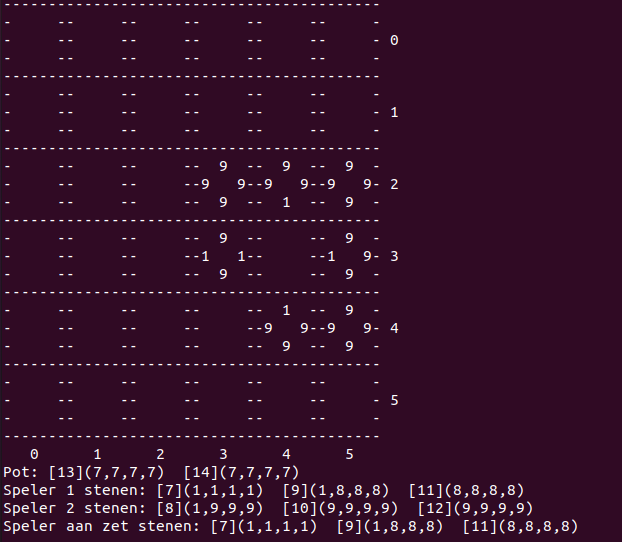
\includegraphics[width=8cm]{algo1/imgs/one.png}
    \caption{Beginsituatie}
    \label{fig:galaxy}
\end{figure}
Speler 1 heeft 3 mogelijkheden:

zet 0; steen 7; rotatie 0-3; 3,4;\\

zet 1; steen 7; rotatie 0-3; 3,2;\\

zet 2; steen 9; rotatie 3  ; 3,4;\\

De goede zet zou in dit geval zet 0 zijn, want met deze zet komt de steen in aanraking met 4 andere stenen. Dit is echter niet de beste zet. De goede zet zal in dit geval leiden tot een verlies. Dit is te zien aan het volgende spelverloop\\
\newpage
\subsection{Spelverloop 1}
Speler 1 speelt steen 7; rotatie 0; 3,4\\

\begin{figure}[htp]
    \centering
    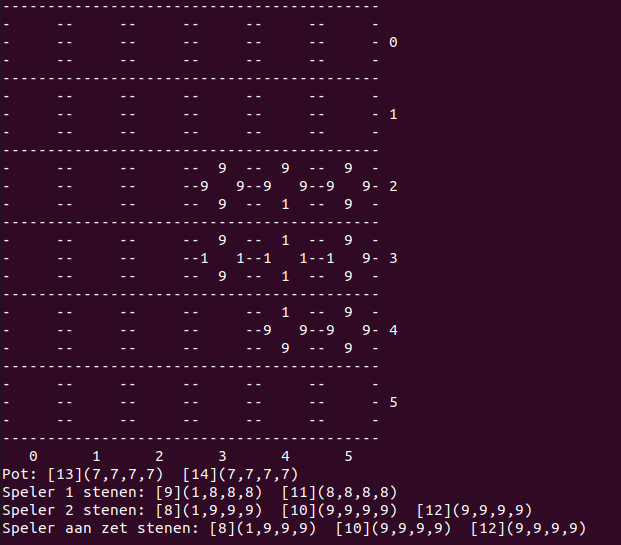
\includegraphics[width=8cm]{algo1/imgs/two.png}
    \caption{Beginsituatie}
    \label{fig:galaxy}
\end{figure}
\newpage

Speler 2 speelt steen 8; rotatie 3; 3,2\\
\begin{figure}[htp]
    \centering
    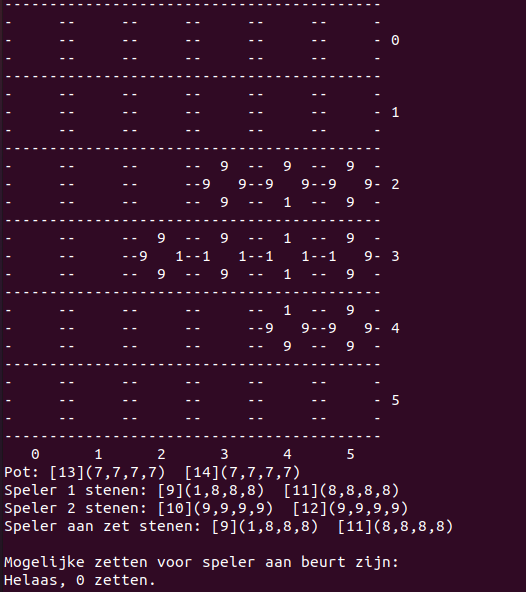
\includegraphics[width=8cm]{algo1/imgs/three.png}
    \caption{Speler 1 kan hierna geen steen meer zetten, en pakt een steen uit de pot maar kan nog steeds geen steen zetten. De beurt wisselt weer terug naar speler 2}
    \label{fig:galaxy}
\end{figure}
\newpage
Speler 2 is weer aan zet\\
\begin{figure}[htp]
    \centering
    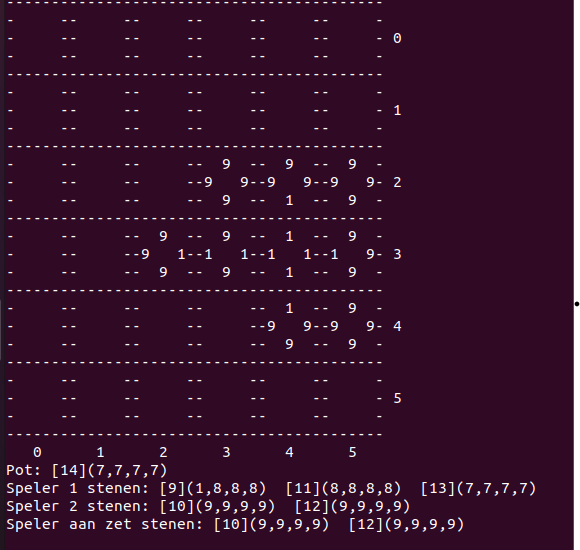
\includegraphics[width=8cm]{algo1/imgs/four.png}
    \label{fig:galaxy}
\end{figure}
\newpage
Speler 2 speelt steen 10; rotatie 0; 1,3
\begin{figure}[htp]
    \centering
    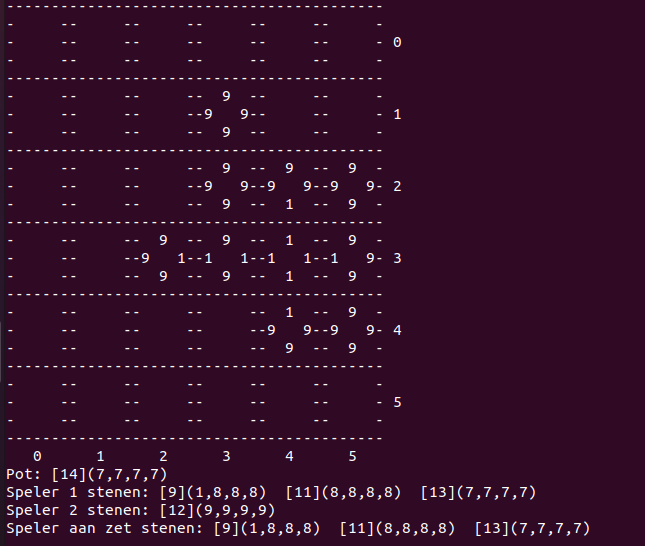
\includegraphics[width=8cm]{algo1/imgs/five.png}
    \caption{Speler 1 kan hierna geen steen meer zetten, en pakt een steen uit de pot maar kan nog steeds geen steen zetten. De beurt wisselt weer terug naar speler 2}
    \label{fig:galaxy}
\end{figure}
\newpage
Speler 2 is weer aan de beurt
\begin{figure}[htp]
    \centering
    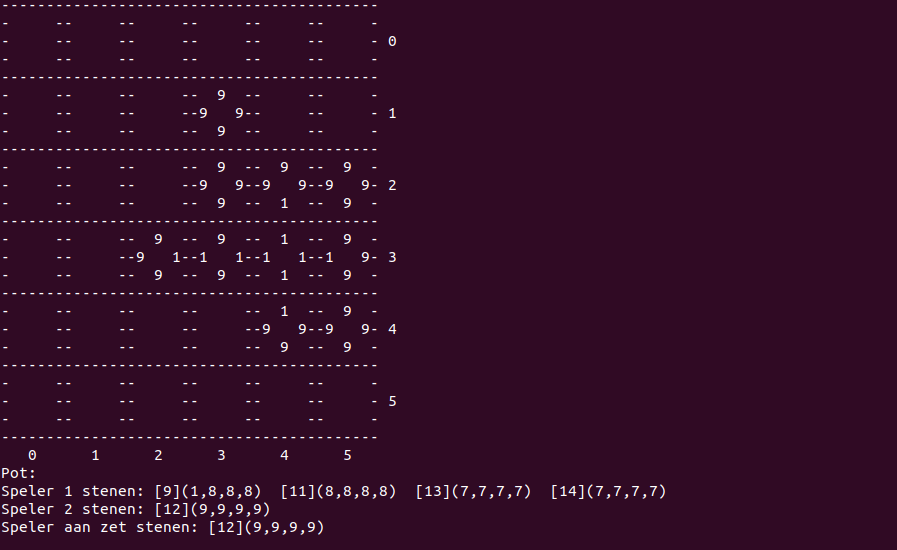
\includegraphics[width=8cm]{algo1/imgs/six.png}
    \label{fig:galaxy}
\end{figure}
\newpage
Speler 2 speelt steen 12; rotatie 0; 0,3
\begin{figure}[htp]
    \centering
    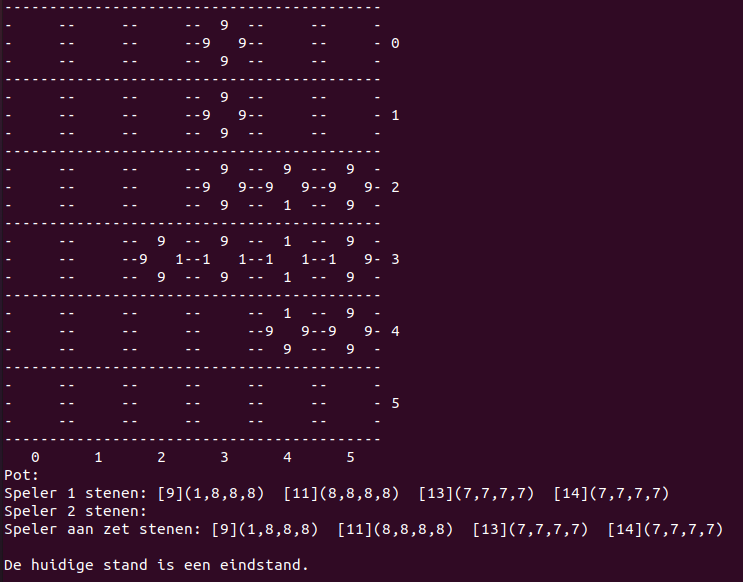
\includegraphics[width=8cm]{algo1/imgs/seven.png}
    \caption{Eindstand is bereikt Speler 2 heeft gewonnen}
    \label{fig:galaxy}
\end{figure}
\newpage 
\subsection{Spelverloop 2}
Als in een alternatief universum, speler 1 anders had gehandeld, dan zou het anders hebben uitgepakt voor speler 2. Zoals in bijvoorbeeld het volgende scenario waarin speler 1 geen "goede" zet speelt.
\begin{figure}[htp]
    \centering
    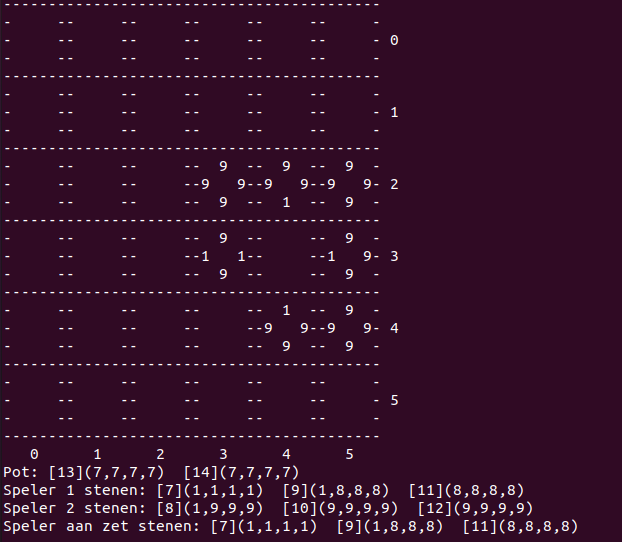
\includegraphics[width=8cm]{algo1/imgs/one.png}
    \caption{Beginsituatie}
    \label{fig:galaxy}
\end{figure}
\newpage
Speler 1 speelt steen 7; rotatie 0; 3,2
\begin{figure}[htp]
    \centering
    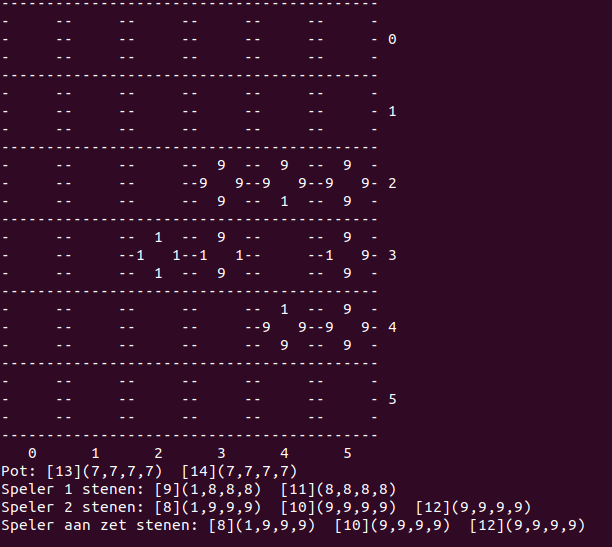
\includegraphics[width=8cm]{algo1/imgs/two_2.png}
    \label{fig:galaxy}
\end{figure}
\newpage
Speler 2 speelt steen 8; rotatie 0; 1,3
\begin{figure}[htp]
    \centering
    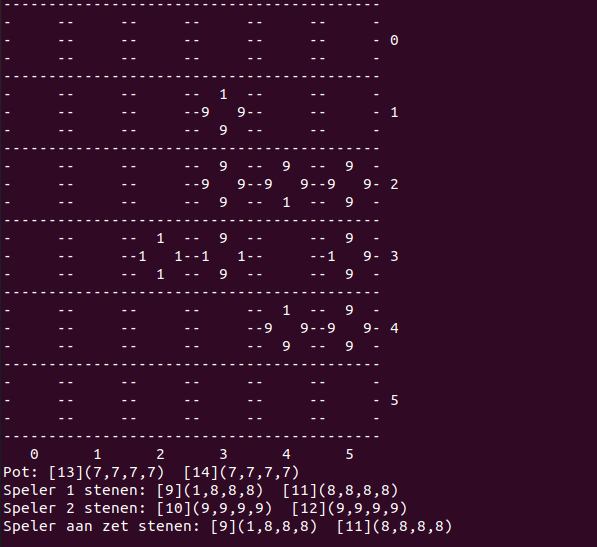
\includegraphics[width=8cm]{algo1/imgs/three_2.png}
    \label{fig:galaxy}
\end{figure}
\newpage
Speler 1 speelt steen 9; rotatie 1; 0,3
\begin{figure}[htp]
    \centering
    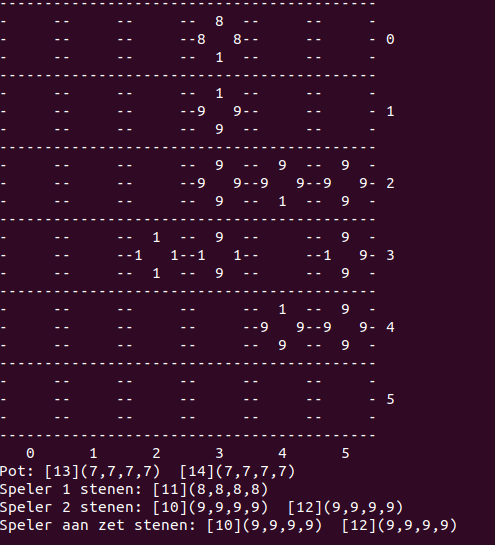
\includegraphics[width=8cm]{algo1/imgs/four_2.png}
    \label{fig:galaxy}
\end{figure}
\newpage
Speler 2 speelt steen 10; rotatie 0; 1,4
\begin{figure}[htp]
    \centering
    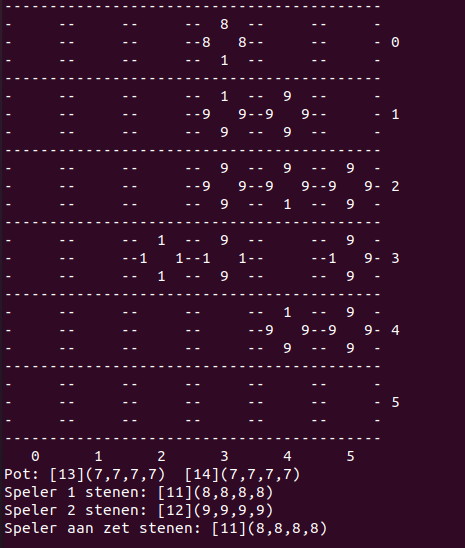
\includegraphics[width=8cm]{algo1/imgs/five_2.png}
    \label{fig:galaxy}
\end{figure}
\newpage
Speler 1 speelt steen 11; rotatie 0; 0,2
\begin{figure}[htp]
    \centering
    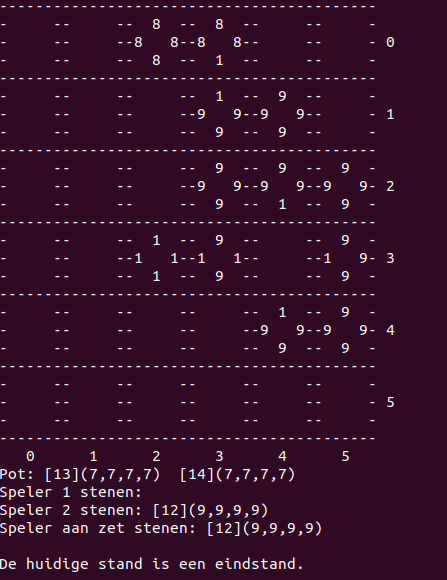
\includegraphics[width=8cm]{algo1/imgs/six_2.png}
    \caption{Eindstand bereikt}
    \label{fig:galaxy}
\end{figure}\\
\\
Speler 1 heeft gewonnen! Speler 1 heeft gewonnen zonder eerst de "goede" zet te spelen in de beginsituatie



\newpage
\section{Experiment}
Dit experiment vergelijkt bij een toenemend aantal stenen de volgende waardes: 
De eindscore voor speler1\\
Het aantal standen dat bekeken is om deze score te berekenen\\
De hoeveelheid tijd die daarvoor nodig is\\
De score voor speler 1 wanneer zij steeds een willekeurige ‘goede zet’ speelt, terwijl
speler 2 steeds een beste zet speelt \\

De resultaten worden opgeslagen in het bestand experiment.txt

Een iteratie van deze functie geeft de volgende resultaten.

\subsection{Resultaten}
\lstinputlisting{experiment.txt}
\newpage

We kunnen met behulp van deze gegevens uitgaan van de volgende beweringen. Des te meer beginstenen er zij. dan:\\
Kan de speler een hogere besteScore behalen\\
Neemt het aantal standen om de besteScore te berekenen exponentieel toe.\\
Neemt de tijd om de besteScore te berekenen exponentieel toe\\ 

Zaken die fout zijn gegaan bij het experiment.

De berekening voor het aantal beginstenen is int(i/4) Dit betekent dat we de getallen achter de komma weg moeten halen, en dat we naar beneden moeten afronden om deze te bereken. De functie round() in cmath had hier beter gebruikt kunnen worden, maar deze headerfile mocht niet worden gebruikt. Dit betekent dat het aantalStanden en de tijd na elk 4tal beginstenen een stuk begint te dalen.\\

De besteScore en scores2 zijn twee verschillende pseudorandom gegenereerde spellen en de waardes tussen elkaar lijken geen enkel verband te hebben, afgezien dat de waardes van score2 gemiddeld gezien lichtelijk hoger zijn. Aan de andere kant kan de berekening van besteScore en score2 verkeerd zijn in welk geval de waardes helemaal nergens op slaan. \\

\section{Appendix}
Alle .h bestanden\\
\subsection{aapjeomino}
\lstinputlisting{aapjeomino.h}
\subsection{zet}
\lstinputlisting{zet.h}
\subsection{standaard}
\lstinputlisting{standaard.h}\\
\\
\\
\section{Alle .cc bestanden}
\subsection{aapjeomino}
\lstinputlisting{aapjeomino.cc}
\subsection{zet}
\lstinputlisting{zet.cc}
\subsection{standaard}
\lstinputlisting{standaard.cc}
\subsection{main}
\lstinputlisting{main.cc}
\section{makefile}
\lstinputlisting{Makefile}
\end{document}
